\documentclass{article}

\usepackage{tikz}
\usetikzlibrary{positioning}
\usetikzlibrary{arrows, automata}
\usetikzlibrary{arrows.meta} 

%\usetikzlibrary{shadows,fadings,shadows.blur}
% install package texlive-pgf-blur to get shadows.blur



\begin{document}


%%%%%%%%%%%%%%%%%%%%%%%%%%%%%%%%%%%%%%%%%%%%%%%%%%%%%%%%%%

%graphframe

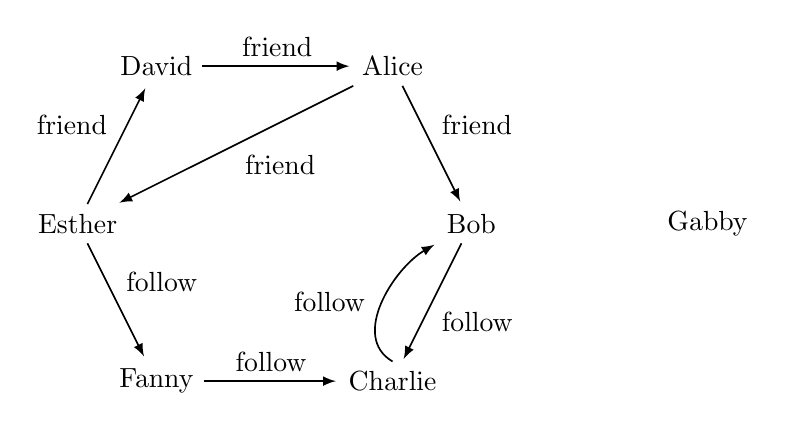
\begin{tikzpicture}[
        > = stealth, % arrow head style
        shorten > = 1pt, % don't touch arrow head to node
        auto,
        node distance = 2cm, % distance between nodes
        semithick % line style
        ]
        
  \node (a) at (4,6) {Alice};
  \node (b) at (5,4) {Bob};
  \node (c) at (4,2) {Charlie};
  \node (d) at (1,6) {David};
  \node (e) at (0,4) {Esther};
  \node (f) at (1,2) {Fanny};
  \node (g) at (8,4) {Gabby};
  \node at (3.2,3) {follow};
  
  \draw[-latex] (a) -- (b) node [midway, fill=white] {friend};
  \draw[-latex] (b) -- (c) node [midway, fill=white] {follow};
  \draw[-latex] (c.north) to [out=150,in=210] (b.south west); 
  \draw[-latex] (f) -- (c) node [midway, fill=white] {follow};
  \draw[-latex] (e) -- (f) node [midway, fill=white] {follow};
  \draw[-latex] (e) -- (d) node [midway, fill=white] {friend};
  \draw[-latex] (d) -- (a) node [midway, fill=white] {friend};
  \draw[-latex] (a) -- (e) node [midway, fill=white] {friend};
  
%\draw [->,red] (4.north) to [out=150,in=30] (1.north);

%\draw (Point1) -- (Point2) node [<position>, fill=white] {Label Text};

\end{tikzpicture}


\newpage


%%%%%%%%%%%%%%%%%%%%%%%%%%%%%%%%%%%%%%%%%%%%%%%%%%%%%%%%%%

%vectorclock

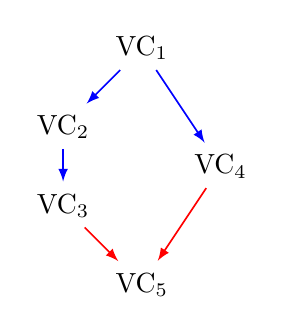
\begin{tikzpicture}[
        > = stealth, % arrow head style
        shorten > = 1pt, % don't touch arrow head to node
        auto,
        node distance = 2cm, % distance between nodes
        semithick % line style
        ]
        
  \node (vc1) at (2,4) {$\mbox{VC}_1$};
  \node (vc2) at (1,3) {$\mbox{VC}_2$};
  \node (vc3) at (1,2) {$\mbox{VC}_3$};
  \node (vc5) at (2,1) {$\mbox{VC}_5$};
  \node (vc4) at (3,2.5) {$\mbox{VC}_4$};
  
  \draw[blue,-latex] (vc1) -- (vc2);
  \draw[blue,-latex] (vc2) -- (vc3);
  \draw[red,-latex] (vc3) -- (vc5);

  \draw[blue,-latex] (vc1) -- (vc4);
  \draw[red,-latex] (vc4) -- (vc5);
  
\end{tikzpicture}


\newpage


%%%%%%%%%%%%%%%%%%%%%%%%%%%%%%%%%%%%%%%%%%%%%%%%%%%%%%%%%%

%graphframe


\begin{tikzpicture}[
        > = stealth, % arrow head style
        shorten > = 1pt, % don't touch arrow head to node
        auto,
        node distance = 2cm, % distance between nodes
        semithick % line style
        ]
        
  \node (a) at (0,0) {};
  \node (b) at (4,0) {};

  \node (texta) at (0,-.5) {vibe coding};
  \node (textb) at (4,-.5) {agentic coding};
  

  \draw[{Circle}-] (0,0) -- (2.2,0);
  \draw[-{Circle}] (1.8,0) -- (4,0);

  
%\draw [->,red] (4.north) to [out=150,in=30] (1.north);

%\draw (Point1) -- (Point2) node [<position>, fill=white] {Label Text};

\end{tikzpicture}








\end{document}



